
\documentclass[12pt, oneside]{article}
\setcounter{secnumdepth}{5}
\usepackage{lmodern} % fuentes
\usepackage[T1]{fontenc} % fuentes
\usepackage[spanish]{babel} % idioma
\usepackage{caption, subcaption} % figuras
\usepackage{graphicx}
\usepackage{array}
\usepackage{amsmath}
\usepackage{mathrsfs}
\usepackage{amsfonts}
\usepackage{amssymb}
\usepackage{physics}
\usepackage{geometry}
\usepackage{mathtools}
\usepackage[width=155mm,top=25mm,bottom=25mm, headheight=15pt]{geometry} % Tamaño de la Página

\begin{document}

\begin{titlepage}
	\setlength{\parindent}{0pt} \setlength{\parskip}{0pt}
	\begin{center}
		\vfill
		
\includegraphics[width=4.5cm]{UNAM_LOGO2.png} \\[1em]
		\Huge\textbf{Universidad Nacional Autónoma de México}
		\vspace{1cm}

		\Large\textbf{Facultad de Ciencias} \\[0.5em]
		Licenciatura en Física
		\vfill

		\Large\textbf{Notas académicas preliminares:} \\
		\large Algoritmo cuántico para la simulación de los estados base del átomo de litio y litio ionizado
		\vspace{1.5cm}

		\textit{Este documento es un fragmento de tesis en desarrollo, de carácter preliminar.} \\
		\textit{No ha sido revisado ni aprobado oficialmente. Queda protegido bajo derechos de autor.}
		\vfill

		\large Emiliano Barragán Bravo \\
		CDMX, México — Agosto 2025
	\end{center}
\end{titlepage}

\section{Introducción}
Aquí irá la introducción del tema, motivación y contexto La computación cuántica nos presenta un futuro prometedor en varias áreas de la física, particularmente representa una gran mejora la simulación de sistemas de química cuántica. En la simulación de los sistemas termiónicos existen dos métodos. El mas antiguo y clásica es la transformación de Jordan-Wigner que permite hacer simulaciones con $O(n)$ operaciones. En años recientes ha aparecido un método alternativo conocido como la transformación de Bravyi-Kitaev el cual permite reducir las operaciones a $O(\log n)$ (ref fermionic quantum computation Bravyi). En el siguiente texto se puede leer cuál es el proceso para la derivación del hamiltonianino para la simulación de una molécula y la aplicación de esta tecnología, en el caso de la simulación de los estados base de una molécula de litio y otra de litio ionizada. Para esto se creará un circuito cuántico utilizando las base de Bravyi-Kitaev utilizando Google Cirq.\\

La motivación de este trabajo es

\subsection{Antecedentes}

Definimos como un spin orbital a la función de onda para un solo electrón. Para su propia definición tenemos que introducir antes los orbitales espaciales. Sea $\psi_i(r)$ una función de la coordenada r talque $\abs{\psi_i(r)}^2dr$ es la probabilidad de encontrar el electrón en un volumen que rodea a la coordenada r. Y por último, para definir un electrón es necesario definir una función spin, que represente el spin 1 y -1, esto lo hacemos con las funciones ortogonales $\alpha(\omega)$ y $\beta(\omega)$. De tal manera que para un grupo de k coordenadas espaciales $\left\{ \psi_i | i=1,..,k\right\}$ tenemos grupo de 2k spines orbitales definidos como:
\begin{equation}
    \begin{split}
        \chi_{2l-1}=\psi_i\alpha(\omega)  \\
        \chi_{2l}=\psi_i\beta(\omega)
    \end{split}
\end{equation}

que cumplen $\braket{\chi_i}{\chi_j}=\delta_{ij}$.\\

\subsubsection{Productos de Hartree y Determinantes de Slatter}

Habiendo definido la función de onda para un electrón, es apropiado considerar la función de onda para múltiples electrones. El producto de Hartree es una respuesta para este caso, este es simplemente la suma de las funciones de onda para cada electrón individualmente i.e.

\begin{equation}
    \Psi(X_1,X_2,...,X_n)=\chi_i(X_1)\chi_j(X_2),...,\chi_k(X_n)
\end{equation}

La cual tiene dos características importantes; Si tomamos $\mathscr{H}$ una eigenfunción de $\Psi(X_1,...,X_n)$, esta cumple que:

\begin{equation}
    \mathscr{H}\Psi(X_1,...,X_n)=E\mathscr{H}
\end{equation}

donde $E=\epsilon_1+\epsilon_2+...+\epsilon_n$ donde definimos $\epsilon_i$ como 

\begin{equation}
    \mathscr{H}\chi_j(X_i)=\epsilon_i\chi_j(X_i)
\end{equation}

además de ser una función independiente, porque cumple que la probabilidad de encontrar el electrón en el volumen $dX_i$ es igual al producto de encontrar cada electron individualmente en cada volume individual:

\begin{equation}
    \abs{\Psi(X_1,...,X_n)}^2dX_1,...,dX_n=\abs{\chi_i(X_1)}^2dX_1+...+\abs{\chi_k(X_n)}^2dX_n
\end{equation}

Los productos de Hartree no cumplen con los principios de antisimétrica de los fermiones. Para resolver este problema se introduce los determinantes de Slatter, esto representan las combinaciones lineales de los productos de Hartree para todos los electrones y espines-orbitales que se tiene. Para el caso de n electrones con k espines orbitales se tiene que el determinante de Slater es (\cite{szabo1996modern}) 

\begin{equation}
    \Psi(\chi_i(X_1),...,\chi_k(X_n))=(N!)^{-1/2}\begin{vmatrix}
        \chi_i(X_1)&\chi_j(X_1)&...&\chi_k(X_1)\\
        \chi_i(X_2)&\chi_j(X_2)&...&\chi_k(X_2)\\
        \vdots&\vdots&\ddots&\vdots\\
        \chi_i(X_n)&\chi_j(X_n)&...&\chi_k(X_n)
    \end{vmatrix}
\end{equation}

\subsubsection{Segunda cuantización}

Iniciamos definiendo a los operadores, creación $a^\dagger$ y aniquilación $a$ como su acción a un determinante de Slatter $a_i^\dagger\ket{\chi_k,...\chi_l}=\ket{\chi_i,\chi_k,...\chi_l}$ y $a_i\ket{\chi_i,\chi_k,...\chi_l}=\ket{\chi_k,...\chi_l}$. Además, estos cumplen que anticomuntan $\{a_i,a_j\}=0$ y  $\{a_i^\dagger,a_j^\dagger\}=0$ i.e. $a_i^\dagger a_j^\dagger=-a_j^\dagger a_i^\dagger$ sí $i=j$ $a_i^\dagger a_i^\dagger=-a_i^\dagger a_i^\dagger$ de igual manera $a_i a_j=-a_j a_i$ y sí $i=j$ $a_i a_i=-a_i a_i$. Esto implica que no podemos crear un electrón en un spin orbital donde ya se encuentra uno y de igual manera no podemos aniquilar un electrón que no existe:

\begin{equation}
    \begin{split}
        a_i^\dagger a_i^\dagger\ket{\chi_j\chi_k}=a_i^\dagger\ket{\chi_i\chi_j\chi_k}=0\\
        a_i a_i\ket{\chi_i\chi_j\chi_k}=a_i\ket{\chi_j\chi_k}=0\\
    \end{split}
\end{equation}

Estos cumplen que la relación entre los operadores cumplen qué $\left\{a_i,a^\dagger_j \right\}=\delta_{ij}$.\\

Para poder definir cualquier operador de slater con estos, operadores es necesario una última definición, el estado vacío, este es el estado en el que no existe ningún electrón, el cual escribiremos como $\ket{0}$ y cumple que:

\begin{equation}
    a_i\ket{0}=0
\end{equation}

Y a partir de este estaco podemos escribir cualquier producto de Hartree, en general:

\begin{equation}
    a^\dagger_i...a^\dagger_k\ket{0}=\ket{\chi_i,..,\chi_k}
\end{equation}

Entonces si consideramos $m$ lugares los cuales pueden estar o no ocupados por una particula fermionica, donde cada sitio lo llamaremos \textit{Local fermionico modes (LFM)}. El espacio de Hilbert definido por este sistema, llamado el espacio de Foch es representado por $2^m$ vectores bases de la forma $\ket{n_0,...,n_j,...,n_{m-1}}$. Todo lo referente a fermiones puede ser representado con los operadores de creacion y aniquilación, estos actuan en los vectores bases de la manera\cite{bravyi2002fermionic}:

\begin{equation}
\begin{split}
    a_j\ket{n_0,...,n_{j-1},1,n_{j+1},...,n_{m-1}}=(-1)^{\sum_0^{j-1}ns}\ket{n_0,...,n_{j-1},1,0,...,n_{m-1}} \\
    a_j\ket{n_0,...,n_{j-1},1,0,...,n_{m-1}}=0
\end{split} 
\end{equation}

Para la representación de nuestro hamiltoniano usaremos el acercamiento de la segunda cuantización. En este acercamiento se hace una suposición esencial conocida como la aproximación de Born-Oppenheimer, en esta se asume que los núcleos están fijos y son solo las dinámicas de los electrones las que se consideran para la simulación. Con esta aproximacion el hamiltoniano electronico de una molécula se define como:

\begin{equation}
    H=\sum_{pq}h_{pq}a^{\dagger}_{p}a_q+\frac{1}{2}\sum_{pqrs}h_{pqrs}a^{\dagger}_{p}a_{q}^{\dagger}a_{r}a_s
\end{equation}

El primer término del hamiltoniano cuenta cada electrón del sistema y por cada uno añade el eigenvalor correspondiente al operador energético (la energía resultante de la energía cinética del electrón y la energía potencial por la interacción entre electrones y del electrón con los protones)de un electrón individual correspondiente a lugar que ocupa en este sistema, y el correspondiente término de $h_{pq}$ es la integral de solapamiento de un electrón. El segundo término del Hamiltoniano corresponde a la transición de dos electrones en los orbitales r y s a los orbitales p y q y $h_{pqrs}$ es la integral de solapamiento de dos electrones\cite{zhang2022quantum}. \\

El Hamiltoniano puede ser representado por el uso de la transformación Bravyi-Kitaev y segunda cuantización. La transformación Bravyi-Kitaev (BKt) es una forma codificar los operadores de creación y aniquilación para un sistema fermionico de manera eficaz. Para definir esta es necesario primero exponer las siguientes bases necesarias.

\section{Transformación de Bravyi-Kitaev}

\subsection{La base de ocupación }

En esta forma de codificar la base electronica del sistema al estado de base de una computadora cuantica, conciste en codificar ocupacion del spin orbital j en el qubit $\ket{q_j}$\\

Por lo tanto,  de manera general la ecuacion de onda de un sistema se codifica como

\begin{equation}
    \ket{f_{n-1},f_{n-2},...,f_1,f_0}\rightarrow\ket{q_{n-1}}\otimes\ket{q_{n-2}}\otimes...\otimes\ket{q_{1}}\otimes \ket{q_0}
\end{equation}

Lo siguiente a hacer es mapear los operador de cracion aniquilacion a operadores de un qubit en esta base i.e. necesitamos construir los operadores $Q^{\pm}$ que cumplan \ref{ecuacion_q_creacion_aniquilacion_ocupationBasis} y agregar una forma de asegurarse que al aplicar los operadores de creacion y aniquilacion se respete el principio de exclusion de pauli

\begin{equation}\label{ecuacion_q_creacion_aniquilacion_ocupationBasis}
    \begin{split}
        Q^{+}\ket{0}=\ket{1}\\
        Q^{+}\ket{1}=0\\
        Q^{-}\ket{0}=0\\
        Q^{-}\ket{1}=\ket{0}
    \end{split}
\end{equation}

De las ecuaciones \ref{ecuacion_q_creacion_aniquilacion_ocupationBasis} podemos deducir que los operadores $Q^{\pm}$ en la base de ocupacion son los siguientes.

\begin{equation}\label{q_ocupation_basis}
\begin{split}
    Q^{+}=\ket{1}\bra{0}\\
    Q^{-}=\ket{0}\bra{1}
\end{split}
    \end{equation}

Sustituyendo \ref{q_ocupation_basis} en las ecuaciones \ref{ecuacion_q_creacion_aniquilacion_ocupationBasis}, podemos comprobar que cumplen lo pedido, estas conclusiones son las mismas que las llegadas por \cite{zhang2022quantum}.

\begin{equation}
    \begin{split}
        Q^{+}\ket{0}=\ket{1}\bra{0}\ket{0}=\ket{1}\cdot1=\ket{1}\\
        Q^{+}\ket{1}=\ket{1}\bra{0}\ket{1}=\ket{1}\cdot0=0\\
        Q^{-}\ket{0}=\ket{0}\bra{1}\ket{0}=\ket{0}\cdot0=0\\
        Q^{-}\ket{1}=\ket{0}\bra{1}\ket{1}=\ket{0}\cdot1=\ket{0}
    \end{split}
\end{equation}

Como en compuptacion cuantica es deseable escribir todo los operadores como composiciones de las matrices de pauli. Una forma de escribir las ecuaciones \ref{q_ocupation_basis} en composicion de matrices de pauli es:

\begin{equation}
    \begin{split}
        Q^{+}=\frac{1}{2}\left(\sigma^x-i\sigma^y \right)\\
        Q^{-}=\frac{1}{2}\left(\sigma^x+i\sigma^y \right)
    \end{split}
\end{equation}

El ultimo paso para terminar de construir los operadores de creacion, es encontrar una forma de agragar el principio de exclusion de pauli a los operadores $Q^{\pm}$. Esto se traduce a que buscamos que al aplicar uno de los dos operadores al qubit ocurran uno de dos escenarios. Sise aplica el operador creación en el qubit $j$ y hay un electron en el spin orbital $j$ el sistema pase a un cero a ritmetico, igualmente si aplicamos el operador aniquilacion al qubit $j$ y no hay un electron en el spin orbital $j$ el sistema tiene que pasar un cero aritmetico. En el segundo escenario buscamos que en el caso en el que al aplicar uno de los operadores el estado del qubit j se invierta. Es en este caso en el que el principio de exclusion de pauli es importante, ya que por este la fase del qubit $j$ cambia segun todos los qubit con indice menor a $j$. Por cada qubit de indice menor a $j$ si el estado este es $\ket{1}$ se agrega una fase $-1$ al sistema, en el caso en el que el qubit este en el estado $\ket{0}$ no se agraga ninguna fase, esto acuerdo a las reglas de anticomutacion de los fermiones. Para lograr esto podemos aprovecharnos de la anticonmutacion de las matrices de pauli, de esta regla podemos deducir que $Q^{\pm}$ anticonmuta con la matriz de pauli $\sigma^z$. Entonces nuestros operadores de creacion y aniquilacion en esta fase son el resultado de aplicar $Q^{\pm}$ en el qubit j y aplicar $\sigma^z$ en todos los qubit con indice menor a $j$ i.e. \cite{bravyi2002fermionic}

\begin{equation}
    \begin{split}
        a^\dagger=\mathbf{1}^{\otimes n-j-1}\otimes Q^+\otimes\left[\sigma^{z\otimes j}\right]\\
        ar=\mathbf{1}^{\otimes n-j-1}\otimes Q^-\otimes\left[\sigma^{z\otimes j}\right]\\
    \end{split}
\end{equation}
\subsection{Alternativas a la base de ocupacion}
\subsubsection{Base de paridad}
AL utilizar la base de ocupacion debemos aplicar $\sigma^z$ a todos los qubits de indice menor a j, esta tarea es dificil y toma demasiado recurso, por lo que buscamos una manera de realizar el mismo proceso con una sola aplicacion de $\sigma^z$. El guardar la fase del sistema puede ser conseguido de manera similiar si en lugar de alamcenar la ocupacion del qubit, el qubit j almacena la suma de los estados de todos los qubits con indice menor o igual a j y despues tomar el modulo de 2, de esta manera cada qubit almacena el estado de fase del sistema correspondiente al estado de cada orbital.\\

La transformacion entre bases esta dada por la ecuacion \ref{transformacion_ocupacion_paridad} donde $\ket{p_i}$ representa la cadena de qubits en la base de paridad y $\ket{q_j}$ la cadena de qubits en la base de ocupacion, n representa el numero de orbitales del sistema y $\pi_n$ es una matriz $\left(n\times n\right)$ definide por

\begin{equation}\label{transformacion_ocupacion_paridad}
    \ket{p_i}=\sum_j\left[\pi_{n}\right]_{ij}\ket{q_j}
\end{equation}

\begin{equation}\label{definicion_matriz_pi}
    \left[\pi_n\right]_ij=\begin{cases}
1 & \text{si } i < j, \\
0 & \text{si } i \geq j.
\end{cases}
\end{equation}

Por ejemplo para cambiar la cadena de qubits en la base de ocupación $\ket{10100111}$ a su correspondiente esta cadena en la base de paridad actuamos con $\pi_8$

\begin{equation}
    \begin{bmatrix}
        1&1&1&1&1&1&1&1\\
        0&1&1&1&1&1&1&1\\
        0&0&1&1&1&1&1&1\\
        0&0&0&1&1&1&1&1\\
        0&0&0&0&1&1&1&1\\
        0&0&0&0&0&1&1&1\\
        0&0&0&0&0&0&1&1\\
        0&0&0&0&0&0&0&1
    \end{bmatrix}\begin{bmatrix}
        1\\0\\1\\0\\0\\1\\1\\1
    \end{bmatrix}=\begin{bmatrix}
        1\\0\\0\\1\\1\\1\\0\\1
    \end{bmatrix}
\end{equation}

En esta base el apliacr o no un cambio de fase al aplicar un operador de creacion o aniquilacion solo depende del qubit $\ket{p_{j-1}}$, existen dos casos en general. Cuando el qubit tiene una paridad 0 entonces $\ket{q_j}\equiv\ket{p_j}$ y la creacion o aniquilacion de un electron es quivalente a aplicar $Q^{\pm}$ como en el caso de la base de ocupacion. El segundo caso es cuando la paridad del qubit es 1, en este caso si $\ket{q_j}=\ket{0}\Rightarrow\ket{p_j}=\ket{1}$ y $\ket{q_j}=\ket{1}\Rightarrow\ket{p_j}=\ket{0}$, entonces en este caso para crear un electron en el orbital $j$ debemos aplicar en qubit $j$ $-Q^-$ y en el caso de querer aniquilar un electron se debe aplicar $-Q^+$. Entonces los operadores de creacion y aniqulacion en esta base se pueden escrribir con la composicion de dos qubits \ref{definicion_p_operadores}:

\begin{equation}\label{definicion_p_operadores}
    P_j^{\pm}=Q_j^{\pm}\otimes\ket{0}_{j-1}\bra{0}_{j-1}-Q^\mp_j\otimes\ket{1}_{j-1}\bra{1}_{j-1}
\end{equation}

Haciendo las comprobaciones de que los operadores $P^\pm_j$ cumplan con lo pedido en ambos casos los aplicamos a $\ket{1}_{j-1}$ y $\ket{0}_{j-1}$.

\begin{equation}\begin{split}
    P^{\pm}_j\ket{0}_{j-1}=\left(Q_j^{\pm}\otimes\ket{0}_{j-1}\bra{0}_{j-1}-Q^\mp_j\otimes\ket{1}_{j-1}\bra{1}_{j-1}\right)\ket{0}_{j-1}\\= Q_j^{\pm}\ket{0}_{j-1}\bra{0}_{j-1}\ket{0}_{j-1}-Q^\mp_j\ket{1}_{j-1}\bra{1}_{j-1}\ket{0}_{j-1}\\=Q_j^{\pm}\ket{0}_{j-1}\cdot1-Q^\mp_j\ket{1}_{j-1}\cdot0=Q_j^{\pm}\ket{0}_{j-1}\\
    \Rightarrow P^\pm_{j-1}\equiv Q^{\pm}_{j-1}
\end{split}  
\end{equation}

Como esperabamos cuando el qubit $j-1$ esta en el estado $\ket{0}$ tenemos la equivalencia de $P^\pm_{j}=Q^\pm_{j}$.

\begin{equation}
    \begin{split}
        P^{\pm}_j\ket{0}_{j-1}=\left(Q_j^{\pm}\otimes\ket{0}_{j-1}\bra{0}_{j-1}-Q^\mp_j\otimes\ket{1}_{j-1}\bra{1}_{j-1}\right)\ket{1}_{j-1}\\= Q_j^{\pm}\ket{0}_{j-1}\bra{0}_{j-1}\ket{1}_{j-1}-Q^\mp_j\ket{1}_{j-1}\bra{1}_{j-1}\ket{1}_{j-1}\\=Q_j^{\pm}\ket{0}_{j-1}\cdot0-Q^\mp_j\ket{1}_{j-1}\cdot1=-Q^\mp_j\ket{1}_{j-1}\\
    \Rightarrow P^\pm_{j-1}\equiv -Q^{\mp}_{j-1}
    \end{split}
\end{equation}

Esto comprueba que cuendo el qubit $j_1$ esta en el estado $\ket{1}$, tenemos la equvalencia $P^\pm\equiv -Q^\mp$, notar que el signo menos se debe a que por la paridad del sistema hay un cambio de fase.\\

Como ya mencionamos antes en computacion cuántica es combeniente escribir los operadores como combinación de las matrices de pauli, en este caso la equivalencia de estos operadores con matrices de pauli tomada de \cite{bravyi2002fermionic} son:

\begin{equation}
    P^\pm_{j}=\frac{1}{2}(\sigma^x_j\otimes\sigma^z_{j-1} \mp i\sigma^y_{j})
\end{equation}

\subsubsection{Base de Bravyi-Kitaev}

Con los métodos anteriores tenemos que los algoritmos que mapean los sistemas son de dificultad $O(n)$, con la idea de reducir esta dificultad se plantea la base de Bravyi-Kitaev una combinación de ambas planteadas en \cite{bravyi2002fermionic} logrando una complejidad de $\log(n)$.

En esta base los qubits de indice par e impar tienen una función diferente. Los qubits de indice par $j=2n$ tienen la función de guardar la ocupación del orbital $j$ i.e. $\ket{f_j}\rightarrow\ket{q_j}$, mientras que los qbubits de indice impar guardan información también guarda un grupo de información de qubits adyacentes con indice menor a j, un ejemplo de esto se puede encontrar en la molécula de hidrógeno, cuya codificación se puede ver en \ref{fig:cod-h2}

\begin{figure}[h]
    \centering
    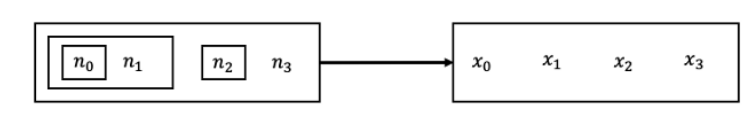
\includegraphics[width=0.5\linewidth]{imagenes//img-transformacion-de-bravyi/codificacion-molecula-de-hidrogeno.png}
    \caption{Codificación de una molécula de hidrógeno en la base de Bravyi-Kitaev, recuperada de \cite{zhang2022quantum}}
    \label{fig:cod-h2}
\end{figure}

En la imagen \ref{fig:cod-h2} los estados de los cuatro orbitales están dado por $\ket{n_0},\ket{n_1},\ket{n_2},\ket{n_3}$ y los correspondientes qubit en la base de Bravyi-Kitaev son $\ket{x_0},\ket{x_1},\ket{x_2},\ket{x_3}$. Entonces las siguientes relaciones se presentan

\begin{equation}
    \begin{split}
        \ket{x_0}\rightarrow\ket{n_0 \text{ mod 2}}\\
        \ket{x_1}\rightarrow\ket{(n_0+n_1)\text{ mod 2}}\\
        \ket{x_2}\rightarrow\ket{n_2 \text{ mod 2}}\\
        \ket{x_3}\rightarrow\ket{(n_0+n_1+n_2+n_2)\text{ mod 2}}
    \end{split}
\end{equation}

Al igual que con la base de paridad el mapeo a esta base se puede representar con una matriz $\beta_n$, llamada la matriz de Bravyi-Kitaev que actúa en una cadena de qubits en la base de ocupación y la transforma a una cadena de qubits en la base de Bravyi-Kitaev, donde al igual que en la base de paridad se asume el mod 2, entonces

\begin{equation}
    \ket{b_i}=\sum_j\left[\beta_n\right]_{ij}\ket{q_j}
\end{equation}

La matriz $\beta_n$ esta definida como:

\begin{figure}
    \centering
    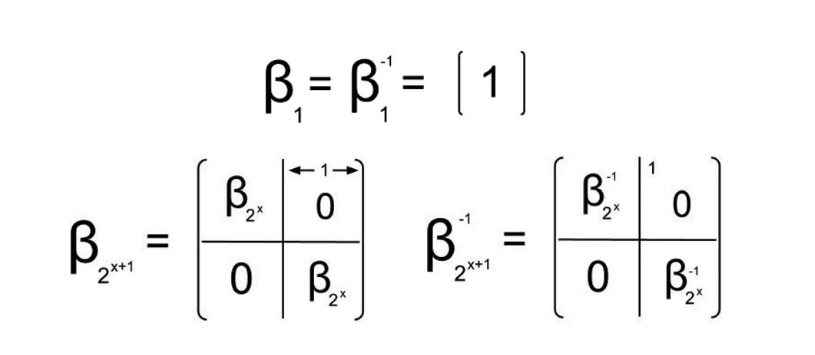
\includegraphics[width=0.5\linewidth]{imagenes//img-transformacion-de-bravyi/definicion-matrix-beta.png}
    \caption{Definición de la matriz $\beta_n$. recuperada de \cite{Seeley_2012}}
    \label{definicion-matriz-beta}
\end{figure}

El caso inicial $\beta_1$ es una matriz $\left(1\times1\right)$ con una sola entrada 1. Subsecuente iteraciones de dimensiones pares de estas matrices de tamaño $n=2^x$ son construidas tomando $1\otimes\beta_{2^{x-1}}$ y llenando la ultima fila con unos 1. En el caso en que las dimensiones de la matriz no sean par i.e. $2^x<n<2^{x+1}$ la matriz $\beta_n$ es el segmento $(n \times n)$ de la matriz $\beta_{2x+1}$ que incluye $b_0$ a $b_{n-1}$ \cite{Seeley_2012}.\\

Un ejemplo de esto es el la transformación del string de bits en la base de ocupación $\ket{10010001}$ a la base de Bravyi-Kitaev aplicando la matriz $\beta_8$.



\begin{equation}
\renewcommand{\arraystretch}{1.2}
\setlength{\arraycolsep}{4pt}
\begin{array}{c@{\hskip 10pt}c}
% Top column labels
& \begin{array}{cccccccc}
    f_7 & f_6 & f_5 & f_4 & f_3 & f_2 & f_1 & f_0
  \end{array}
\\[0.1em]
% Row labels + actual matrix
\begin{array}{c}
  b_7 \\
  b_6 \\
  b_5 \\
  b_4 \\
  b_3 \\
  b_2 \\
  b_1 \\
  b_0 \\
\end{array}
&
\left(
\begin{array}{cccccccc}
1 & 1 & 1 & 1 & 1 & 1 & 1 & 1 \\
0 & 1 & 0 & 0 & 0 & 0 & 0 & 0 \\
0 & 0 & 1 & 1 & 0 & 0 & 0 & 0 \\
0 & 0 & 0 & 1 & 0 & 0 & 0 & 0 \\
0 & 0 & 0 & 0 & 1 & 1 & 1 & 1 \\
0 & 0 & 0 & 0 & 0 & 1 & 0 & 0 \\
0 & 0 & 0 & 0 & 0 & 0 & 1 & 1 \\
0 & 0 & 0 & 0 & 0 & 0 & 0 & 1 \\
\end{array}
\right)
\left(
\begin{array}{c}
1 \\
0 \\
0 \\
1 \\
0 \\
0 \\
0 \\
1 \\
\end{array}
\right)
=
\left(
\begin{array}{c}
1 \\
0 \\
1 \\
1 \\
1 \\
0 \\
1 \\
1 \\
\end{array}
\right)
\end{array}
\end{equation}

Por lo tanto la transformacion del bit de string a la nueva base es entonces $\ket{10010001}\rightarrow\ket{10111011}$.\\

Antes de definir los operadores de creación y aniquilación es necesario mostrar como el aplicar estos operadores modifica de manera diferente a tres grupos de qubits. Con estos grupos podremos definir de manera directa los operadores de creación y aniquilación.

\subsubsection{Grupo de paridad}

\end{document}
